% proposal.tex
\documentclass[main.tex]{subfiles}
\begin{document}
\chapter{Proposed Work} \label{ch:proposal}

The use of AM technologies to produce small batches of highly customized, complex parts, in a reduced development cycle results extremely attractive. While constructing failure envelopes can help overcome the wariness of industrial segments to design end-user parts, this resource is still not easy to implement, requiring a large number of mechanical tests and specialized equipment to properly map the failure behavior of a particular material. Additional complexity stems from what was shown in Section \ref{sec:SSICAM}: processing the same material under related AM technologies yields completely different failure envelopes, implying that no generalizations should be made, and each material-process pairing needs to be studied on a case-by-case basis. In general, for AM parts to be adopted, engineers have to be able to confidently assess the probability of part failure under particular loading conditions, predict the expected mechanical properties of AM parts, and understand the underlying physics of the process. None of these considerations are completely understood at the time of this work. The solutions presented in this proposal are aimed at solving one of these three issues. This work aims to provide the tools required to understand and predict properties and mechanical performance of parts manufactured through FFF. Some, if not all of the procedures developed in this work could even be extrapolated to other AM techniques. The end goal is having the framework necessary to streamline the development of failure envelopes for FFF as much as possible, making a compelling case for adoption of this technology in the production of end user parts subjected to complex loading conditions. 

\section{Objectives} \label{sec:objectives}

The set of printing conditions that lead to an optimal part in terms of mechanical properties aren't still fully comprehended. However, if there existed an FFF machine with in-line sensors that allowed monitoring a variety of process-variables, as well as data generated from mechanical tests and ancillary experiments, this would constitute an interesting case for development of a Machine Learning (ML) system. These excel in cases where the inputs and outcomes of a particular phenomena or task are known, but connecting the two through an explicit set of rules or relationships can result extremely complex and time consuming \cite{Chollet2018}. In this manner, ML models are \emph{trained}, as opposed to explicitly programmed, as illustrated in Figure \ref{fig:MLvsP}, where the differences between ML and traditional programming philosophies are compared. 

\begin{figure}[!htbp]
	\center
	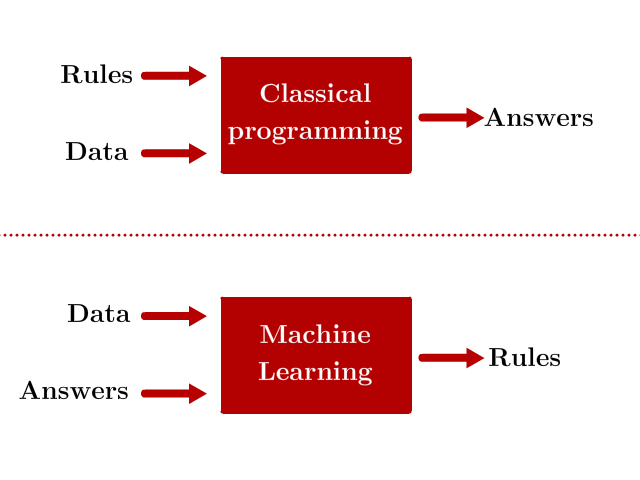
\includegraphics[height=6.5cm]{ML}
	\caption{Differences between traditional programming and machine learning. \cite{Chollet2018}} \label{fig:MLvsP}
\end{figure}

The fundamental goal of this research is to predict FFF part mechanical performance by finding relations between processing conditions and strength through the use of sensors and machine learning. The success of this project would allow design engineers to confidently assess if a part manufactured through FFF will meet the mechanical requirements imposed by its intended application. This work proposes developing and using a modified printer with force and print speed sensors, as well as mechanical testing and $\mu$CT scans to generate data that can be used to train a predictive tool based on ML. This tool can then be used to predict final mechanical properties of the part based on the data generated during the print. This ML system would accept filament dimensions, printing temperature, filament force, filament velocity, print orientation, or any subset of these items as inputs, and produce final part porosity and mechanical strength in a particular load direction as outputs. These parameters were chosen based on previous work performed by Koch, Van Hulle and Rudolph \cite{Koch2017}, where the final tensile strength of FFF coupons was shown to be related to the morphology of the printed bead, which is significantly affected by processing parameters and variations in the volumetric output of the nozzle, as well as the proposed FFF melting models established by Bellini \emph{et al.} \cite{Bellini2004} and Osswald \emph{et al.} \cite{OsswaldMelting18}. The specifics of the architecture of the ML system are still under development, as it may prove useful to segment the problem into several sub-systems connected in series, in what is called a machine learning \emph{pipeline} \cite{Geron2019}. However, given the specifics of the task, one can conclude that the system will involve supervised learning applied to a regression problem, given that all the inputs to the system will consist of pre-selected attributes, and the mechanical response and/or porosity of a printed part can be treated as a target value the ML system has to be able to predict.

\begin{figure}[!htbp]
	\center
	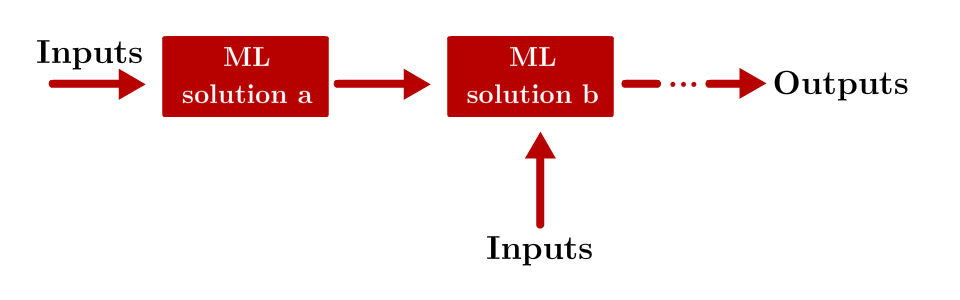
\includegraphics[height=3.5cm]{ML2}
	\caption{Pipeline architecture for advanced ML systems \cite{Geron2019}} \label{fig:pipeline}
\end{figure}

\section{Preliminary results} \label{sec:prelim}

Preliminary work for this study involved designing and deploying a 3D Printer capable of capturing filament force and extrusion velocity mid-print. An FFF machine was developed in collaboration with FusedForm (Bogot\'{a}, Colombia) based on their simplest model: the FusedForm Minilab. The printer was equipped with a customized force sensor and a thermistor built into the printhead, as well as an encoder that records the extruded filament length through time. The concentric force sensor was positioned just above the hot end in a bowden extruder architecture. These modifications permit recording and visualization of live force, speed, and temperature data during the printing process, while maintaining the original performance and functionality of the 3D printer intact. The generated data is then collected using an Arduino board connected to MATLAB for visualization, processing and logging. A schematic representation of the machine can be seen in Figure \ref{fig:shakira}, where dashed lines represent the path followed by the filament, and the dotted lines represent the signal sent to the Arduino board.

\begin{figure}[!htbp]
	\center
	\includegraphics[height=7.5cm]{forcesetup}
	\caption{Schematic of modified FFF printer with sensors} \label{fig:shakira}
\end{figure}

An initial set of experiments, designed to capture trends in filament force and velocity during a controlled print was designed. Two materials were chosen: a customized ABS filament, extruded in-house, and a commercially available PLA filament, each with a diameter of 1.75 mm. The ABS filament was produced using the SABIC Cycolac™ MG94 material. This is an ABS resin traditionally used for injection molding thin walled parts, as well as FFF filament. With a reported Melt Flow Index of 11.7 g/10 min, it is an ideal resin for both the FFF and extrusion processes \cite{sabic2016}. The extrusion setup consisted of a single screw extruder (Extrudex EDN 45X30D, Germany) with 45 mm screw diameter and L/D ratio of 30D. The hot melt was extruded at 205 ºC through a circular die with a 4.2 mm diameter. It was then guided through a pre-skinner into a vacuum-assisted, heated water bath (Conair, USA) to cool the extrudate whilst minimizing void formation. The solidified filament then passes through a 3-axis laser micrometer (LaserLinc, USA) and a belt puller (Conair, USA) in a control loop that allows adjustment of the pull speed to keep the extrudate within specification. The desired filament dimensions were a diameter of 1.75 mm with a tolerance of ± 0.02 mm. The PLA filament used was the commercially available "Natural PLA PRO" filament sold by Matterhackers \cite{MH2020}, chosen to minimize the effect of colorants/additives to the composition of the filament. Steps were taken to ensure that all the acquired spools of material came from the same lot as to guarantee that processing conditions during the extrusion process were constant. A laser micrometer was used to extract information pertaining to filament geometry, as seen in Figure \ref{fig:FD}.

\begin{figure}[!htbp]
	\center
	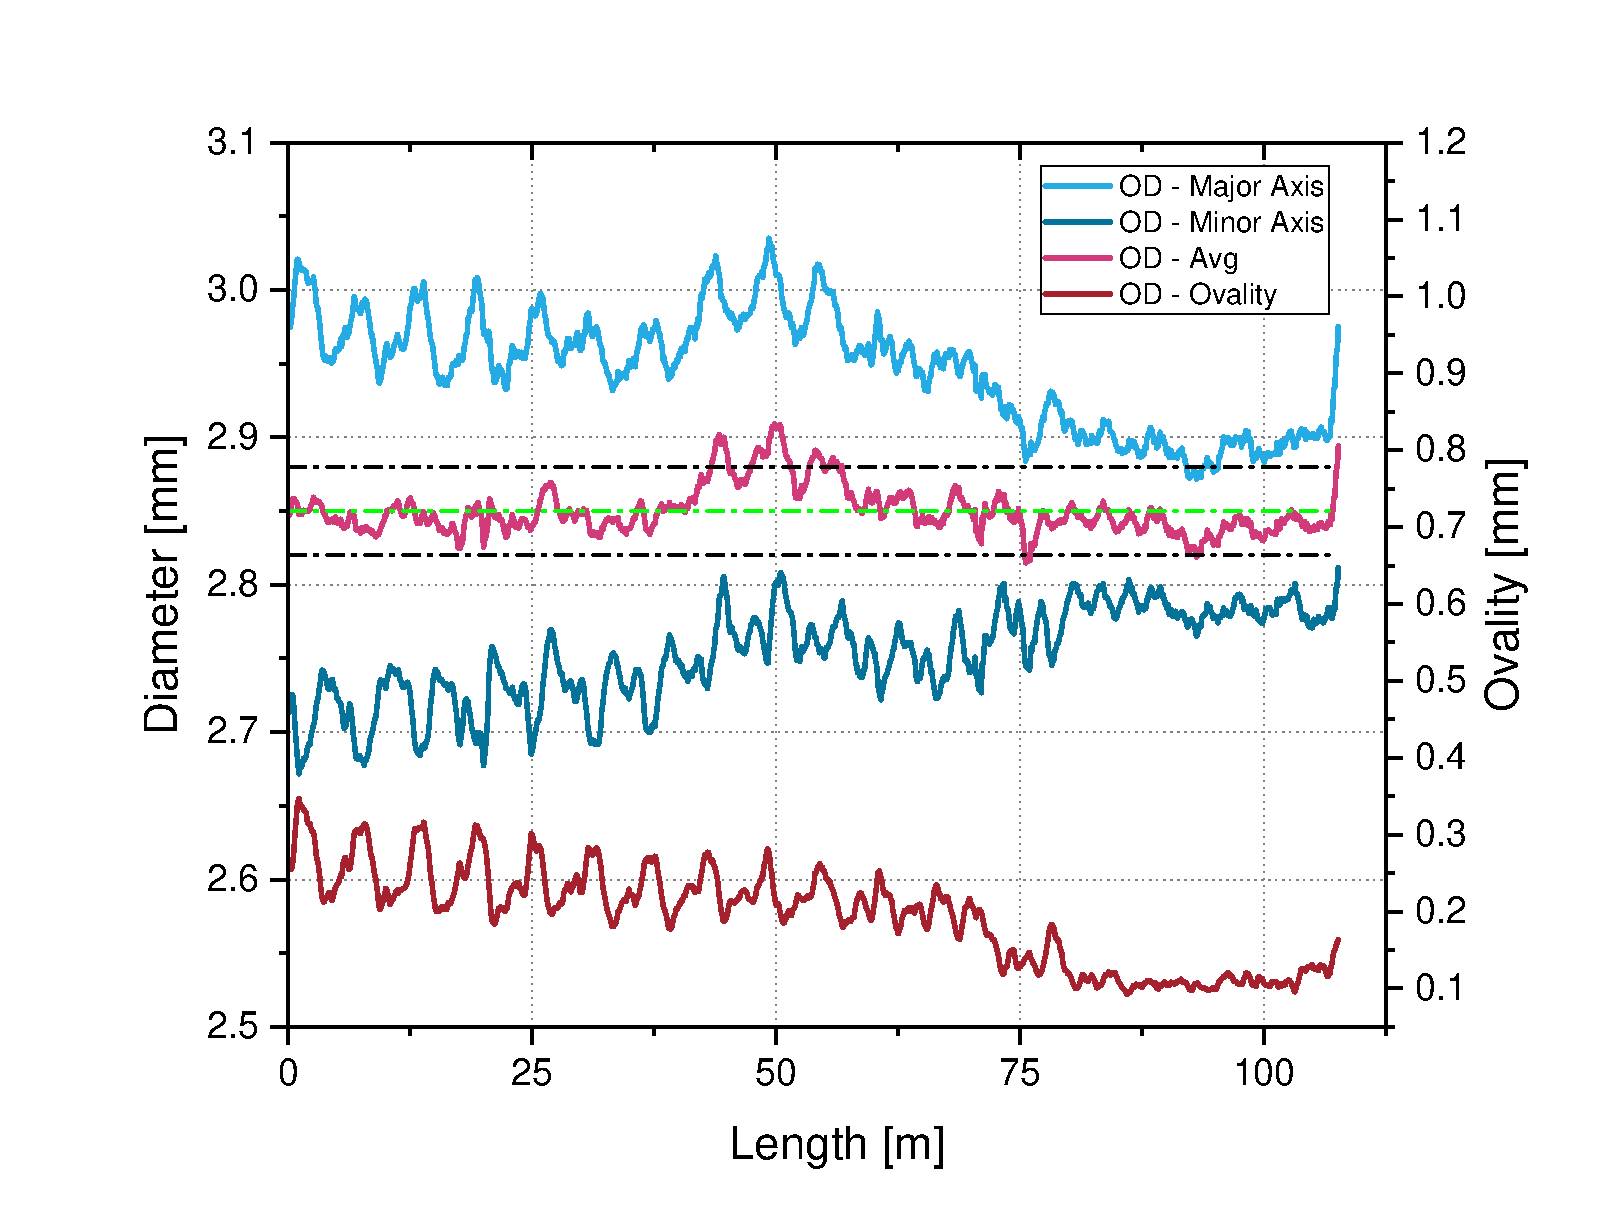
\includegraphics[width=0.8\linewidth]{FD.pdf}
	\caption{Filament geometry information, acquired through a laser micrometer } \label{fig:FD}
\end{figure}

In order to explore the effect of printing temperature and print speed upon stable printing conditions in terms of required filament force, several toolpath files were developed, where the print velocity varied was varied in increments of 5 mm/s every 15 layers, each with a thickness of 0.35 mm. To minimize the effects of varying accelerations during the test, a cylindrical geometry with a radius of 75 mm, printed in continuous helical mode was chosen as the benchmark part. This ensures that changes in filament force and velocity stem mostly from the extrusion process and not due to toolpath considerations. To verify the effect of print temperature upon the required extrusion force, each material was printed at three different temperatures: 200, 215 and 230°C for PLA, and 215, 230 and 245°C for ABS. 

\begin{figure}[!htbp]
	\center
	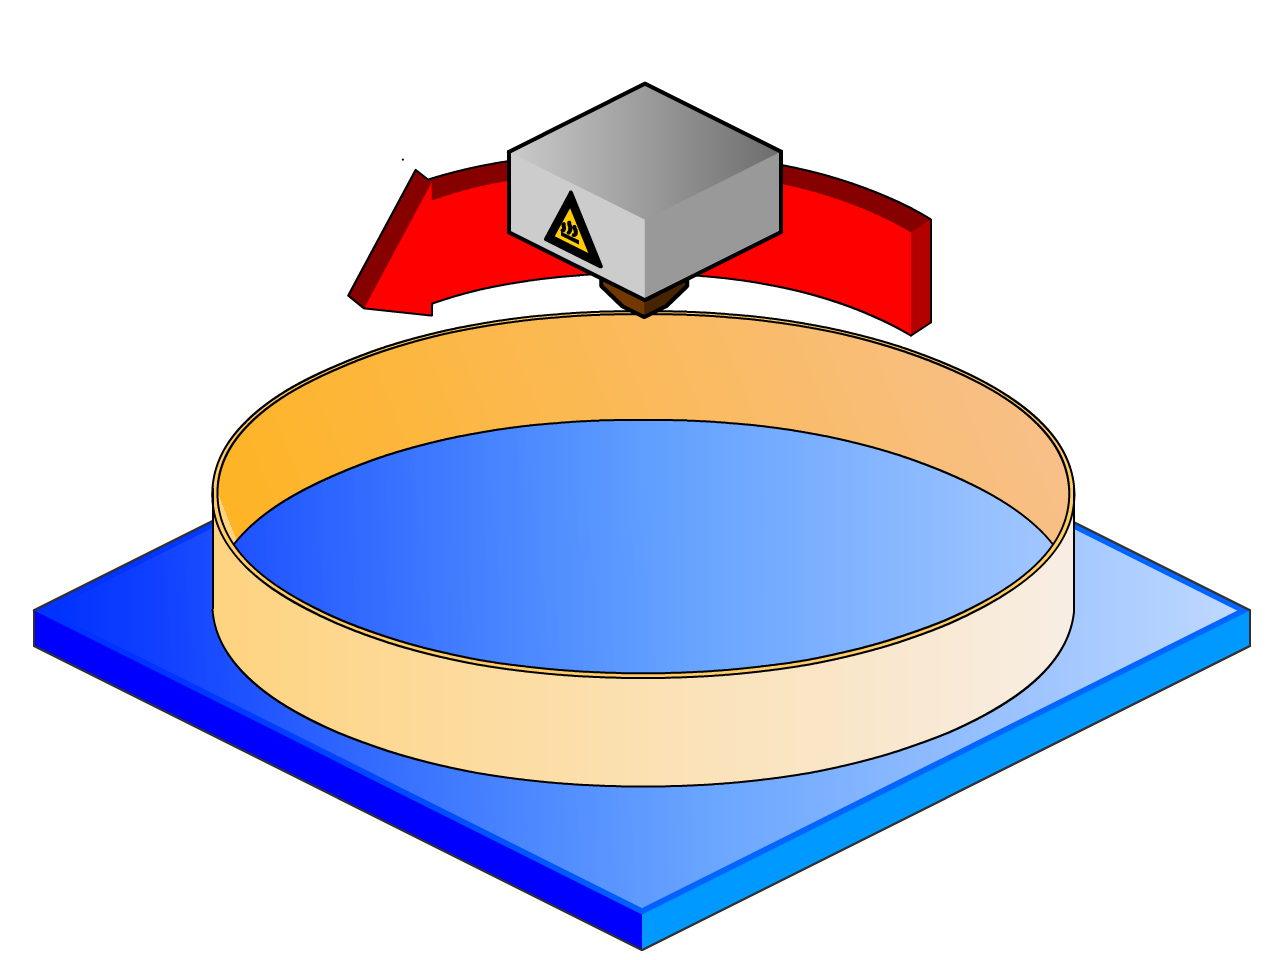
\includegraphics[width=0.8\linewidth]{cyl_shakira}
	\caption{Continuous print for force-velocity data collection} \label{fig:cyl}
\end{figure}

\begin{figure}[!htbp]
	\center
	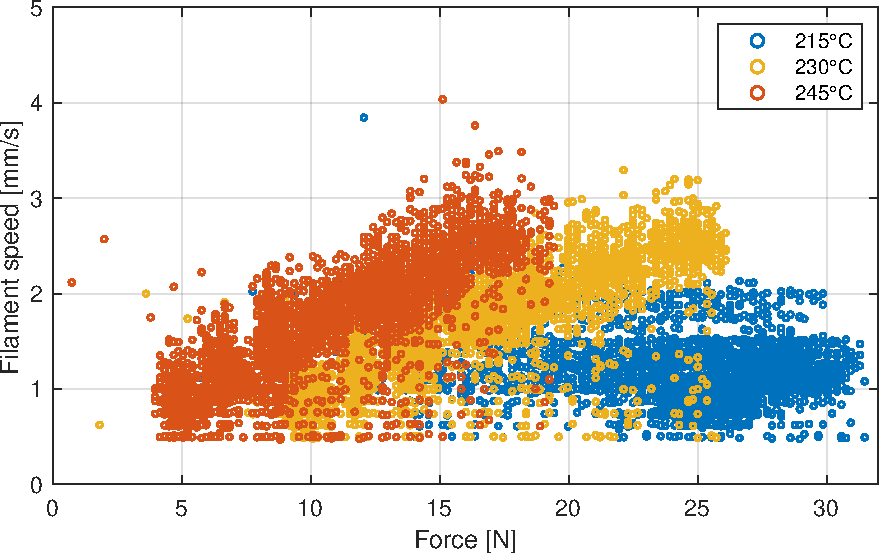
\includegraphics[width=0.8\linewidth]{ABS_prelim.pdf}
	\caption{Comparison of Force requirements for ABS} \label{fig:absprelim}
\end{figure}

\begin{figure}[!htbp]
	\center
	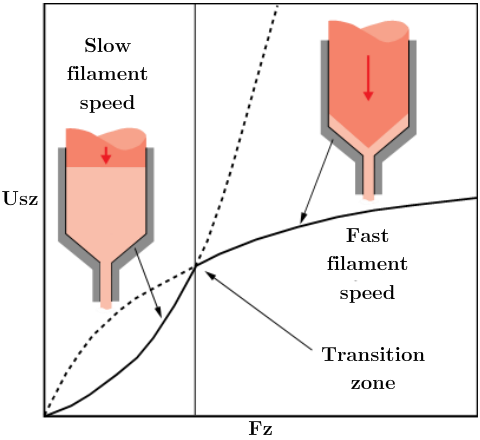
\includegraphics[width=0.7\linewidth]{meltmodes}
	\caption{Potential explanation for extrusion force-velocity trends} \label{fig:meltmodes}
\end{figure}



\section{Future work} \label{sec:fw}



%__________________________________________________________________________________________________________
% Nomenclature introduced in this chapter:
\nomenclature[A]{ML}{Machine Learning}% 

% Symbols introduced in this chapter:
\nomenclature[S]{$X_t$}{Tensile strength in the 1-1 direction \nomunit{$MPa$}}
\end{document}